\chapter{Requisitos del proyecto}

El objetivo que persigue este capítulo es definir todos los requisitos que ha de cumplir el proyecto. Se establecerá la nomenclatura utilizada para nombrar  cada requisito de forma inequivoca. Después, para cada una de las partes en las que ha sido dividido el proyecto, la librería y el videojuego, se detallarán uno a uno dichos requisitos.

\newpage

%%%%%%%%%%%%%%%%%%%%
%              PACMAN GAME                   %
%%%%%%%%%%%%%%%%%%%%

\section{Nomezclatura}

Cada requisito del proyecto vendrá identificado mediante la siguiente notación:
$$Nombre del proyecto : Módulo : Índice$$
\begin{itemize}
\item El nombre del proyecto se corresponderá con `TFC', las siglas de `Trabajo Fin de Carrera'.
\item El módulo se corresponde con `PACMAN' si es un requisito del videojuego o con 'LIB' si es un requisito de la librería.
\item Por último, el índice será un valor número autoincremental.
\end{itemize}

Tras haber definido cómo se van a identificar los requisitos, en las siguientes secciones  se irán describiendo uno a uno. El objetivo que se persigue con estos requisitos es fijar el alcance final de proyecto con la mayor exactitud posible.

\section{Requisitos del videojuego}
\begin{description}
\req {TFC:PACMAN:001} {El flujo de pantallas de la aplicación se define en el gráfico de la figura 5.1 que se muestra en la página siguiente.

	\begin{figure}[p]
	\centering	
         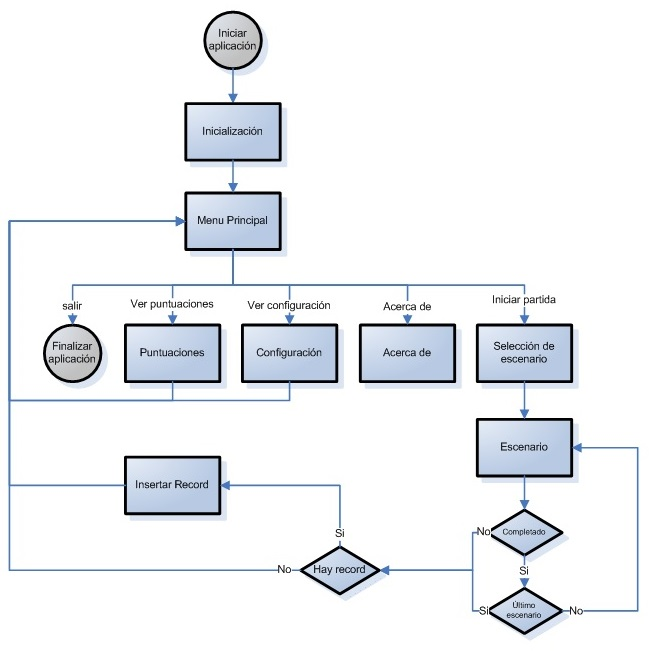
\includegraphics[width=15cm]{img/EstructuraGeneralPacmania.jpg}
	\caption{Estructura general de la aplicación}
	\end{figure}
}

\req{TFC:PACMAN:002} {Al iniciar la aplicación se mostrará la pantalla de 'Inicialización' en la cual, se irá indicando las acciones realizadas por la aplicación, entre ellas, lecturas de ficheros, cargas de imágenes\ldots
}

\req{TFC:PACMAN:003} {Al finalizar en proceso de carga de la aplicación, se cambiará automáticamente de la pantalla de 'Inicialización' a la pantalla de 'Menú principal'. Sobre el menú principal se podrán realizar las siguientes acciones:
\begin{multicols}{2}
\begin{itemize}
\item Acerca de                  
\item Configuración             
\item Iniciar partida         
\end{itemize}
\begin{itemize}
\item Marcadores               
\item Salir del programa
\item []
\end{itemize}
\end{multicols}

Cada una de las acciones tiene asociado un cambio de pantalla, que se describirá en posteriores requisitos. El flujo de estas acciones está descrito en el gráfico primer requisito funcional TFC:PACMAN:001.
}

\req {TFC:PACMAN:004} {La opción 'Acerca De', ubicada en el menú principal, abrirá una ventana emergente que mostrará la siguiente información.
\begin{multicols}{2}
	\begin{itemize}
	\item Autor del proyecto
	\item Tutor del proyecto
	\item Universidad
	\end{itemize}
	\begin{itemize}
	\item Facultad
	\item Año de realización
	\item []
	\end{itemize}
\end{multicols}
}

\req {TFC:PACMAN:005} {La opción 'Marcadores', ubicada en el menú principal, mostrará una nueva ventana con las diez mejores partidas realizadas en el videojuego y en el smartphone donde ha sido instalada la aplicación. 

Cuanto mejor ha sido una partida mayor puntuación habrá obtenido, por lo tanto, se ordenaran de mayor a menor puntuación. 

En cada posición se indicará un texto con el nombre de la persona que consiguió el récord, y la puntuación lograda.
}

\req{TFC:PACMAN:006} {La opción 'Configuración', ubicada en el menú principal, mostrará una nueva ventana en la cual se permitirá establecer los siguientes criterios:
\begin{itemize}
\item Sonido: indica si el sonido del juego está encendido o apagado.
\item Path: directorio donde se encuentran los ficheros de configuración.
\item Módulo: listado de escenarios que compondrán el videojuego. Los posibles módulos a cargar están ubicados en el directorio de configuración.
\end{itemize} 
}

\req{TFC:PACMAN:007} {La opción 'Iniciar Partida', ubicada en el menú principal, mostrará una nueva ventana, en la cual se mostrarán los distintos escenarios que contiene el modulo cargado. 
El usuario podrá seleccionar cualquiera de ellos, al hacerlo, se cargará el escenario seleccionado.
}

\req{TFC:PACMAN:008} {Al finalizar el escenario el sistema comprobará si se ha realizado con éxito, si es así, se cargará el siguiente escenario definido en el módulo. 

En el caso de no haber completado con éxito el escenario actual o de no existir más escenarios se volverá al menú principal. 

Si la puntuación obtenida está entre las diez mejores, antes de volver al menú principal, aparecerá una ventana para indicar el nombre asociado a ese nuevo récord. 
}

\req{TFC:PACMAN:009} {Cada escenario contendrá los siguientes elementos: 
	\begin{itemize}
	\item Pacman: elemento dinámico que será manejado por el usuario.
	\item Fantasmas: elementos dinámicos gestionados por la computadora cuyo objetivo es capturar al Pacman.
	\item Pastillas: elementos estáticos que han de ser recogidos por el Pacman.
	\end{itemize}
}

\req{TFC:PACMAN:010} {El Pacman puede realizar dos tipos de movimientos, los cuales se pueden simultanear:
	\begin{itemize}
	\item Desplazamientos sobre el plano XY, es decir, sobre una cuadrícula, por lo tanto siempre son horizontales o verticales.		
	\item Desplazamientos sobre el plano Z que se corresponden con saltos y junto con un desplazamiento en el eje X o Y implicará un tiro parabólico.
	\end{itemize}
}

\req{TFC:PACMAN:011} {En cualquier momento el Pacman podrá cambiar el sentido del movimiento, incluso cuando se este produciendo un salto. }

\req{TFC:PACMAN:012} {La dirección de un elemento sólo podrá cambiar en los cruces de la cuadrícula.}

\req{TFC:PACMAN:013} {Ninguno de los elementos del juego podrán atravesar las paredes del escenario.}

\req{TFC:PACMAN:014} {Los fantasmas únicamente tendrán la posibilidad de realizar movimientos sobre el eje XY, por lo tanto no saltarán.}

\req{TFC:PACMAN:015} {Los posibles algoritmos asociados al comportamiento automático de un fantasma son los siguientes:
	\begin{itemize}
	\item Aleatorio: se elegirá una dirección al azar en la que se moverá el fantasma en el siguiente cruce.
	\item Persecución: seguirá el camino mínimo existente en el escenario entre su posición y la del Pacman.
	\end{itemize}
}

\req{TFC:PACMAN:016} {Los fantasmas podrán cruzarse entre sí, por lo que no se realizará ninguna acción cuando colisionen.} 

\req{TFC:PACMAN:017} {Al iniciar una partida el usuario tiene cero puntos y tres vidas u oportunidades para superar todos los escenarios.}

\req{TFC:PACMAN:018} {Cuando el Pacman choca contra una pastilla, ésta desaparece del escenario y se incrementa la puntuación en el marcador en 10 unidades.}

\req{TFC:PACMAN:19} {Cuando el Pacman choca contra una fantasma se pierde una vida.  } 

\req{TFC:PACMAN:20} {El escenario se dará por finalizado cuando el Paman haya recogido todas las pastillas contenidas en él.}

\req{TFC:PACMAN:21} {La partida finaliza bajo dos situaciones:
	\begin{itemize}
	\item El usuario pierde todas las vidas. 
	\item El usuario completa todos los escenarios del módulo.
	\end{itemize}
}

\req{TFC:PACMAN:22} {La partida podrá pausarse en cualquier momento.}

\req{TFC:PACMAN:23} {Se permitirá pausar el videojuego en el trascurso de un escenario. Si el videojuego está en pausa, el escenario cambiará su color a escala de sepias.}

\req{TFC:PACMAN:024} {Ha de crearse un módulo llamado "Pacmania", compuesto por los siguientes niveles: 
	\begin{figure}[!h]
		\centering	
		\subfloat[Primer nivel del módulo]{
			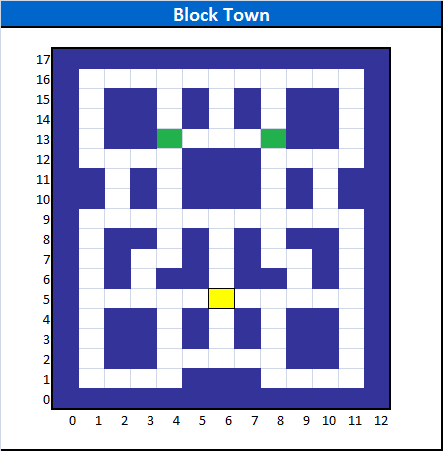
\includegraphics[height =6.5cm]{img/Esquema_BlockTown.jpg}
		}
		\subfloat[Segundo nivel del módulo]{
			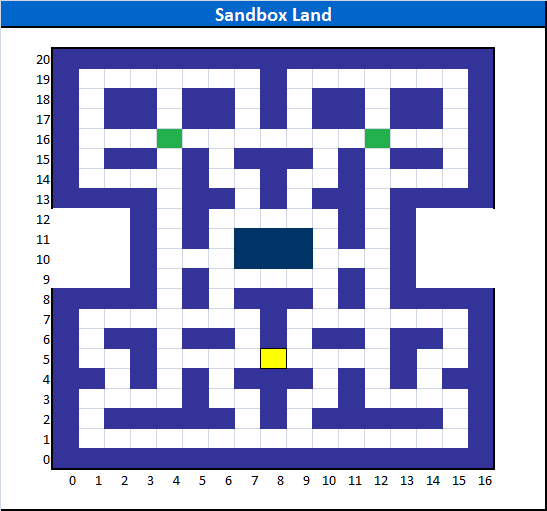
\includegraphics[height =6.5cm]{img/Esquema_SandboxLand.png}
		}
	\end{figure}

	Sobre cada uno de los escenarios se identifica:
	\begin{itemize}
		\item El cuadrado amarillo identifica la posición inicial de Pacman.
		\item Los cuadrados azules son las paredes del escenario
		\item Los cuadrados verdes son las posiciones iniciales de los fantasmas.
	\end{itemize}
}

\req{TFC:PACMAN:025} {Al finalizar todos los niveles del módulo se mostrará un vídeo de fin de partida completada.}

\req{TFC:PACMAN:026} {Al perder todas las vidas se mostrará un vídeo distinto de fin de partida no completada.}

\req{TFC:PACMAN:027} {Antes de mostrar cada escenario se procederá a mostrar un vídeo introductorio.}

\req{TFC:PACMAN:028} {Cada escenario tendrá asociada una melodía que se escuchara de fondo, durante el transcurso de la partida, en dicho escenario.}

\req{TFC:PACMAN:029} {Cada módulo ha de tener una melodía que se escuchará desde el principio del juego hasta seleccionar un escenario. 
A partir de ese momento será sustituida por la melodía del escenarios seleccionado.}

\req{TFC:PACMAN:030} {Al chocar con una pastilla se realizara un sonido.}

\req{TFC:PACMAN:031} {Al perder una vida se reproducirá un sonido.}

\req{TFC:PACMAN:032} {Durante la partida, la cámara irá siguiendo los movimientos del Pacman.}

\req{TFC:PACMAN:033} {Al empezar cada escenario se realizará un efecto de acercamiento con la cámara hacia el Pacman.}

\req{TFC:PACMAN:034} {Al perder una vida se realiza una animación girando la cámara 720 grados.}
\end{description}

%%%%%%%%%%%%%%%%%%%%
%                  LIBRERIA                       %
%%%%%%%%%%%%%%%%%%%%

\section{Requisitos de la librería}
\begin{description}

\req{TFC:LIB:001}{Se adaptará el componente gráfico de OpenGL para Android, llamado GLSurfaceView, dotándole de funciones especificas de un videojuego. Cuando el sistema operativo refresque la pantalla se realizarán las siguientes acciones.
	\begin{itemize}
	\item Calcular el tiempo transcurrido desde la última actualización.
	\item Obtener nuevas posiciones de los distintos elementos del escenario. Se han de tener en cuenta las propiedades de los distintos elementos y el tiempo transcurrido.
	\item Ejecutar un pre-render que permita al programador ampliar con nuevas funcionalidades el componente gráfico.
	\item Actualizar el escenario en pantalla con la nueva información calculada.
	\end{itemize}
  }

\req{TFC:LIB:002}{La estructura de datos a partir de la cual se definirá el escenario estará compuesta por:
	\begin{itemize}
	\item Nombre y descripción de la escena.
	\item Una cámara.
	\item Malla del escenario.
	\item Listado de elementos que componen la escena.
	\end{itemize}
}

\req {TFC:LIB:003}{Los comportamientos posibles de una cámara son:
	\begin{itemize}
	\item \textbf{Estático:} La cámara no se mueve.
	\item \textbf{Programada:} La cámara sigue una trayectoria previamente configurada mediante rotaciones sobre los ejes y los puntos inicial y final. Para dicho comportamiento también se han de indicar la velocidad lineal y angular.
	\item \textbf{Persecutoria:} La cámara sigue a un elemento del juego desde una distancia predeterminada.
	\item \textbf{Compuesta:} La cámara realiza una composición de los comportamientos mencionados.
	\end{itemize}
}


\req {TFC:LIB:004}{La estructura de datos que determina la información de un elemento de la escena esta compuesta por:
	\begin{itemize}
	\item Las coordenadas de su posición en el escenario.
	\item Propiedades físicas de cinemática para creación de movimiento rectilíneos uniformes en un espacio tridimensional.
	\item Aspecto gráfico del elemento.
	\item Forma implícita.
	\item Comportamiento del elemento, en el cual se determina si es gestionado de forma manual o bajo inteligencia artificial.
	\item Deteccción de colisiones automáticas habilitado.
	\end{itemize}
}

\req{TFC:LIB:005}{La algoritmos de inteligencia artificial disponibles, determinando el comportamiento de un elemento, son los siguientes:
	\begin{itemize}
	\item \textbf{Manual:} el usuario interactúa con el juego describiendo trayectorias sobre la pantalla, las cuales indican hacia donde debe moverse el elemento.
	\item \textbf{Aleatorio:} el elemento se mueve sobre el escenario cambiando su dirección y sentido de forma aleatoria.
	\item \textbf{Dijkstra:} el elemento se mueve por la ruta mas corta hacia un determinado punto.
	\end{itemize}

	Todos estos comportamientos se basan en movimientos sobre una cuadrícula.
}

\req {TFC:LIB:006}{Las formas implícitas de los elementos del juego se definen mediante superficies de contorno de tipo AABB o la composición de las mismas.}

\req{TFC:LIB:007}{El comportamiento ante colisiones de un elemento puede ser \textbf{Fuerte} o \textbf{Débil}. El comportamiento fuerte sólo ha de asociarse a elementos que, cuando existas una colisión con ellos, no tengan acciones asociadas en el videojuego, pudiendo ser delegadas directamente a la libreria. El ejemplo más claro son las paredes de un escenario, cuando un elemento choque con ellas, la única acción a realizar es resolver la colisión.
} 

\req{TFC:LIB:008}{El motor del videojuego calculará las colisiones existentes cada vez que se actualice el componente gráfico de Android. Las colisiones que tengan un elemento cuyo comportamiento sea fuerte, se resolverán situando el elemento con comportamiento débil, justo antes de que se produjera la colisión. }

\req{TFC:LIB:009}{El aspecto gráfico de cada elemento ha de estar determinado por uno de los siguientes tipos de mallas:
	\begin{itemize}
	\item \textbf{TextureShaderMesh:} se corresponde con elementos cuyo apariencia está representada por una malla, teniendo en cuenta los vértices, las caras, los vértices de la textura y las texturas.
	\item \textbf{ParticleShaderMesh:} se corresponde con un elemento que esta compuesto por partículas\footnote{Todas las pastillas del juego son representadas por un único elemento de tipo ParticleShaderMesh. Cada pastilla se corresponde con un vértice o partícula de este tipo de mallas, permitiendo, con una sola invocación a la tarjeta gráfica, dibujar todas las pastillas del escenario de forma óptima.}, cada una de ellas equivale a un vértice de la malla que se representará con un punto.
	\item \textbf{AnimatedShaderMesh:} se corresponde con elementos cuya apariencia se asocia con una secuencia de mallas, de esta forma es posible la creación de animaciones sin necesidad de usar esqueletos.
	\end{itemize}
}

\req {TFC:LIB:010}{La librería tendrá una utilidad que permitirá leer ficheros Wavefront (.obj y .mtl) para generar mallas de tipo TextureShadersMesh. 

Este tipo de fichero son generados a partir del la aplicaciones de diseño 3D como Blender y 3D Studio, las cuales son usadas a nivel profesional para crear  películas de animación y videojuegos.}

\req{TFC:LIB:011}{El motor de juegos no implementará ningún modelo de iluminación. Los efectos provocados por las luces sobre los elementos del videojuego, serán procesados previamente en sus texturas, a partir de las aplicaciones de diseño 3D.

La generación de texturas que incluyen la iluminación de la escena se conoce como `cocinar las texturas' (\texttt{Texture Bake}).
}

\req{TFC:LIB:012}{La librería permitirá reproducir dos tipos de sonidos:
	\begin{itemize}
	\item Una única melodía, que se corresponder con la música de fondo de una pantalla.
	\item Los efectos especiales que se corresponden con los distintos sonidos que se producen en el videojuego, como por ejemplo colisiones entre los distintos elementos, alcanzar ciertas puntuaciones\ldots
	\end{itemize}
}

\end{description}